\documentclass{lni}

\IfFileExists{latin1.sty}{\usepackage{latin1}}{\usepackage{isolatin1}}

\usepackage{graphicx}


\author{
	Nikolaus Moll\footnote{Bis 31.12.2012 Student im Master-Studiengang Informatik / akademischer Mitarbeiter der HTWG Konstanz; seit 01.02.2014 t\"atig bei der Pentasys AG in München. E-mail: nikol@usmoll.de}\\ Christian Baranowski, J\"urgen W\"asch \\ 
	\\ 
	Fakult\"at Informatik,
	HTWG Konstanz \\ 
%	Brauneggerstrasse 55 \\ 
%	D-78462 Konstanz \\ 
%	nikol@usmoll.de %\\
%	\{tzink, haase, waesch\}@htwg-konstanz.de
}
\title{Modellierung und Generierung von Test-Daten f�r Datenbank-basierte Anwendungen\footnote{Die Arbeit wurde im Kontext des FHprofUnt-Projektes ''Transparente Integration von NAT-Traversierungstechniken in Java'' durchgef\"uhrt, das vom BMBF und der Seitenbau GmbH in Konstanz gef\"ordert wird. Projektpartner sind die HTWG Konstanz, Seitenbau GmbH und die Universit\"at Konstanz.}}
\begin{document}
\maketitle




\begin{abstract}
Softwaretests haben sich als Teil der Qualit�tssicherung von Softwareprojekten etabliert.
F�r Tester ist die Modellierung von Testdaten f�r Datenbank-basierte Anwendungen allerdings
nicht immer einfach. Die Daten k�nnen aufgrund von Beziehungen von Datens�tzen schnell
un�bersichtlich und komplex werden. Wegen der Komplexit�t versuchen Tester, mehrere Tests
mit denselben Daten durchzuf�hren.

In dieser Masterarbeit werden eine neue Modellierungssprache f�r Testdaten f�r
Datenbank-basierte Anwendungen und ein Algorithmus zur Generierung von Testdaten 
vorgestellt. Die Sprache erlaubt eine �bersichtliche Beschreibung von Daten und
von Beziehungen zwischen Datens�tzen. Der Algorithmus zur Generierung erzeugt
Daten anhand der Beziehungstypen im Datenbank-Modell. Der Algorithmus versucht
viele Grenzf�lle zu erzeugen, so dass die Daten in m�glichst vielen Tests verwendet
werden k�nnen.
\textit{Apache License 2.0}.

\end{abstract}


\section{Problemstellung und Überblick}

%Softwaretests sind ein wichtiger Baustein f�r die Qualit�tssicherung von modernen Softwareprojekten.
%F�r Tests werden Testdaten spezifiziert. Auf deren Basis wird das Verhalten der Software gepr�ft.
%Bei Datenbank-basierten Anwendungen werden Testdaten in der Regel sehr umfangreich und komplex.
%
%Die Komplexit�t ergibt sich aus der Beschreibung von Beziehungen zwischen den einzelnen
%Datens�tzen. Besonders bei Systemen mit komplexen Datenbank-Schemata kann ein
%Testdaten-Modell schnell un�bersichtlich werden.
%
%F�r den Tester sind un�bersichtliche Testdaten aus verschiedenen Gr�nden ein Problem.
%Einerseits machen sie die Pflege fehleranf�llig. Andererseits ist es schwer,
%die modellierten Daten zu erfassen und zu verstehen. Tester w�nschen deshalb h�ufig Daten,
%die f�r mehrere Tests nutzbar sind. Dadurch reicht es aus, nur ein oder zumindest
%wenige Daten-Modelle zu verstehen und zu pflegen.
%
%Die im Rahmen einer Master Thesis [Quelle] entwickelte Modellierungssprache f�r Testdaten erlaubt
%eine �bersichtliche Modellierung von Testdaten. Sie ist einfach zu nutzen und integriert sich
%in g�ngige Entwicklungsumgebungen.
%
%Dar�ber hinaus wurde ein Algorithmus f�r die Generierung von Testdaten konzipiert. Das Ziel des
%Generators ist es, mit wenigen Datens�tzen viele Grenzf�lle bei Beziehungen abzudecken.



%
%\textbf{Aus FORUM Artikel}
%
%Zum Testen von Software-Anwendung, die Daten persistent in einem Datenbanksystem verwalten, werden Testdaten für die Datenbank benötigt. Für Anwendungen mit einem komplexen Datenbankschema ist die Spezifikation dieser Testdaten meist nicht trivial, da neben den Entitäten auch deren Beziehungen betrachtet werden müssen. Diese Beziehungen unterliegen in der Regel einer Menge komplexer fachlicher Regeln, die sich aus dem Domänen-Modell der Anwendung ergeben. 
%
%In dieser Arbeit wird untersucht, wie die zum Test von Datenbank-basierten Anwendungen notwendigen Testdaten auf einfache Weise beschrieben und automatisch erzeugt werden können.
%
%%---
%
%Eine zu prüfende Anwendung wird im Kontext von Software-Tests als System under Test (SUT) bezeichnet. Alle Voraussetzungen für einen Test werden dabei als sog. Test Fixture bezeichnet. Idealerweise soll die in einem Test Fixture beinhaltete Datenmenge für einen funktionalen Test eine hohe Testabdeckung bieten, dabei aber so klein und übersichtlich wie möglich sein. Somit sind die Testdaten einfacher zu verstehen und für eine große Anzahl von funktionalen Tests zu verwenden.
%
%Ein üblicher Ansatz, ein SUT in Verbindung mit einer Datenbank zu testen, ist das Testmuster Back Door Manipulation \cite{XUNIT_TEST_PATTERNS}. Idee hierbei ist, dass das Einspielen des Test Fixture in die Datenbank direkt durch den Test am SUT vorbei, d.h. sozusagen durch eine Hintertür, geschieht. Im ersten Schritt, dem Setup, wird die Datenbank über direkten Zugriff an dem SUT vorbei in den Anfangszustand des Test Fixture gebracht. Anschließend können im Exercise-Schritt die zu testenden Operationen am SUT durchgeführt werden. Die Überprüfung, ob sich das SUT richtig verhalten hat, findet im Verify-Schritt statt. Dabei kann der Zustand der Datenbank mit dem erwarteten Zustand des SUT verglichen, ebenfalls über die Test-eigene Datenbankverbindung. Abschließend können im vierten optionalen Schritt, Teardown, noch Aufräumarbeiten in der Datenbank implementiert sein.
%
%Basis für die nachfolgend beschriebenen Projektarbeiten ist die Java-Bibliothek Simple Test Utils for JUnit \& Co. (STU) zur Vereinfachung von Unit-Tests für Java-Anwendungen. STU steht unter der Apache License 2.0 und wird von der Firma Seitenbau entwickelt. Für Tests von Datenbank-basierten Anwendungen setzt STU auf der Bibliothek DbUnit [2] auf. DbUnit ist ein Framework zum Testen von Datenbank-basierten Java-Anwendungen. 
%
%Ziel des Projekts ist es u.a., funktionale Tests durch die Spezifikation eines Java-API und einer speziellen Testdatenbeschreibungssprache so zu vereinfachen, dass eine Datenbank einfach zu Beginn des Tests – über den Test selbst – in den wohldefinierten Anfangszustand das Test Fixture versetzt werden kann. Des Weiteren soll der erwartete Datenbank-Zustand am Testende einfach auf Basis des Test Fixture beschrieben werden können. Nach Ausführung des Tests soll automatisch der über das SUT erzeugte Datenbank-Zustand mit dem erwarteten Datenbank-Zustand verglichen und somit die Korrektheit der Anwendung geprüft werden können.

%%%----

%Alle Voraussetzungen für einen Test werden dabei als sog. Test Fixture bezeichnet. 
%%
%Idealerweise soll die in einem Test Fixture beinhaltete Datenmenge für einen funktionalen Test eine hohe Testabdeckung bieten, dabei aber so klein und übersichtlich wie möglich sein. Somit sind die Testdaten einfacher zu verstehen und für eine große Anzahl von funktionalen Tests zu verwenden.
%
%
%
%Ein üblicher Ansatz, ein SUT in Verbindung mit einer Datenbank zu testen, ist das Testmuster Back Door Manipulation \cite{XUNIT_TEST_PATTERNS}.
%
%Alle Voraussetzungen für einen Test werden dabei als \emph{Test Fixture} bezeichnet.
%%
%Ein üblicher Ansatz, ein SUT in Verbindung mit einer Datenbank zu testen, ist das Testmuster Back Door Manipulation \cite{XUNIT_TEST_PATTERNS}. Im Setup wird die Datenbank über direkten Zugriff an dem SUT vorbei in den Anfangszustand des Test Fixture gebracht. Anschließend können im Exercise-Schritt die zu testenden Operationen am SUT durchgeführt werden. Die Überprüfung, ob sich das SUT richtig verhalten hat, findet im Verify-Schritt statt. Dabei kann der Zustand der Datenbank mit dem erwarteten Zustand des SUT verglichen, ebenfalls über die Test-eigene Datenbankverbindung. 
%%Abschließend können im vierten optionalen Schritt, Teardown, noch Aufräumarbeiten in der Datenbank implementiert sein.

%%%%%---


Softwaretests sind ein wichtiger Baustein für die Qualitätssicherung von Softwareprojekten. Für Tests von Datenbank-basierten Anwendungen müssen u.a.~Testdaten für die Datenbank spezifiziert werden, auf deren Basis das Verhalten der zu testenden Software 
%(System Under Test, SUT) 
geprüft werden kann.
%
%
Die Spezifikation dieser Testdaten ist leider augenblicklich sehr umfangreich und komplex und somit aufwändig und fehleranfällig.
%
%Bei datenbank-basierten Anwendungen sind die Testdaten meist sehr umfangreich und komplex.
%
Die Komplexität ergibt sich v.a.~aus der Beschreibung der Beziehungen zwischen den einzelnen Entitäten.
%im Test Fixture.
%
Diese unterliegen einer Menge komplexer fachlicher Regeln, die sich aus dem Domänen-Modell und der Geschäftslogik der Anwendung ergeben.
%
%%%Besonders bei Systemen mit großen oder komplexen Datenbank-Schemata kann ein Testdaten-Set schnell unübersichtlich werden.


Übergreifendes Ziel der hier beschriebenen Arbeit \cite{MT:Moll:2013} war es, die Spezifikation von Testdaten für Datenbank-basierte Java-Anwendungen zu vereinfachen.
%
Hierzu wurde zum einen  eine geeignete Domänen-spezifische Sprache (DSL) für Testdaten entwickelt.
%
%%%Die DSL erlaubt eine  übersichtliche Spezifikation von Testdaten, ist einfach zu nutzen und integriert sich in gängige Entwicklungsumgebungen.
%
Zum anderen wurde ein Generator zur automatischen Erzeugen von Testdaten implementiert. 
%
%%%Das Ziel hierbei war es, mit möglichst wenig Datensätzen viele Grenzfälle bei Beziehungen abzudecken.
%
%
Basis der Entwicklungsarbeiten war die Java-Bibliothek Simple Test Utils for JUnit \& Co. (STU) zur Vereinfachung von Unit-Tests für Java-Anwendungen.
%
STU steht unter der Apache License 2.0 und wird federführend von der  SEITENBAU GmbH entwickelt. 
%
%%%Für Tests von Datenbank-basierten Anwendungen setzt STU auf der Bibliothek DbUnit auf.


\begin{figure}[tb]
	\begin{center}
		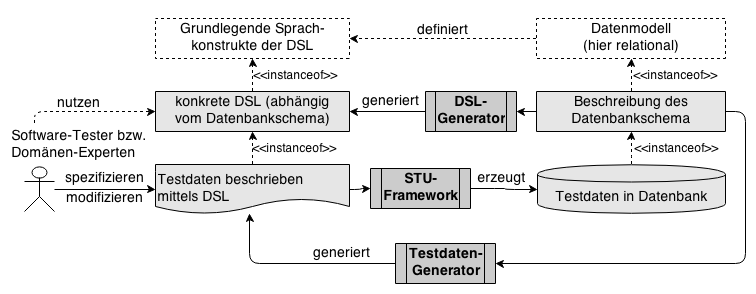
\includegraphics[width=12.75cm]{images/ansatz.png}
		\caption{\label{ansatz}Überblick über den gewählten Ansatz.}
	\end{center}
   %\vspace{-0.5cm}  %%% BAD HACK JW
\end{figure}

Abb.~\ref{ansatz} gibt einen Überblick über den gewählten, modellgetriebenen Ansatz.
%
Ausgangspunkt ist eine formale Beschreibung des relationalen Datenbankschemas (Details siehe \cite{MT:Moll:2013}).
%
Diese kann mittels eines Tools (nicht dargestellt) manuell erstellt bzw.~aus einer existierenden Datenbank extrahiert und ergänzt werden.
%
Aus der Schema-Beschreib\-ung wird die schema-abhängige Testdaten-DSL generiert. 
%
Diese DSL kann dann von den Testern genutzt werden, um verschiedene Testdaten-Sets zu beschreiben und diese mittels STU in ihre Unit-Tests einzubinden.
%
Die Testdaten-Sets werden bei den Tests durch das STU-Framework automatisch in die Datenbank eingespielt.
%
%%%(Backdoor-Manipulation \cite{XUNIT_TEST_PATTERNS}). 
%
Auf Basis von der Schema-Be\-schrei\-bung können auch in der DSL beschriebene Test\-da\-ten-Sets  generiert werden. Die generierten Testdaten können ggfls.~vor Verwendung noch angepasst werden.
%
%
%
%Details und ausführliche Code-Beispiele zur Verwendung sind in \cite{MT:Moll:2013} zu finden.





	






\section{Testdaten-DSL}


%\textbf{Aus FORUM Artikel}
%
%Die Spezifikation der Testdaten soll mit Hilfe einer Domänenspezifische Sprache (DSL) und des Java-API erfolgen. Eine DSL ist eine formale Sprache, die speziell für ein bestimmtes Problemfeld, die sogenannte Domäne, entworfen und implementiert wird. Der Entwurf einer DSL soll einen hohen Grad an Problemspezifität erreichen, d.h. die Sprache soll alle Probleme der Domäne darstellen können und nichts darüber hinaus. Dadurch ist die Sprache durch Domänenspezialisten, in unserem Fall z.B. die Software-Tester, ohne besonderes Zusatzwissen leicht nutzbar.
%
%Im Projektkontext bedeutet domänenspezifisch, dass die DSL die grundlegenden Konzepte der Datenbank-Strukturierung (in unserem Fall das relationale Datenmodell) unterstützen muss, aber auch vom fachlichen Datenbankschema abhängig ist, das dem SUT zugrundeliegt.  D.h. für jede zu testende Anwendung wird aus einer erweiterten Spezifikation des zugrundeliegenden Datenbankschemas eine spezielle DSL erzeugt, in der die Testdaten dann durch die Software-Tester bzw. die Domänenexperten beschrieben werden können (siehe Abb. 3).

Es wurden verschiedene Ansätze zur Entwicklung einer DSL für Testdaten untersucht. Der Fokus lag u.a. auf der Fachlichkeit der Datenstruktur, der typsicheren Beschreibung der Testdaten und der einfachen Spezifikation von Beziehungen zwischen Entitäten. Untersucht wurden verschiedene XML-basierte Darstellungen, wie z.B. in DbUnit benutzt, programmatische Spezifikationen und verschiedene tabellarischen Beschreibungsformen für die Testdaten. 
%
Nach einer Evaluation wurde eine tabellarische Beschreibungsform gewählt, die über das STU-Framework genutzt werden kann. Diese Art der Testdatenmodellierung ist übersichtlich, syntaktisch einfach und kann von einer IDE wie Eclipse unterstützt werden. Die grundlegende Idee für die tabellarische Darstellung stammt vom Testframework Spock \cite{Spock}.
%
Die EBNF der DSL ist in \cite{MT:Moll:2013} zu finden.



\begin{figure}[tb]
\begin{lstlisting}[caption=Mittels DSL beschriebenes Testdaten-Set (Table Builder API)., style=java, label=listing:dsl]
class BookDatabaseGroovyDataSet extends BookDatabaseBuilder
{
  <def> tables() {
    `buchTable`.rows {
      @REF@            | @name@
      @CLEANCODE@      | "Clean Code"      
      @EFFECTIVEJAVA@  | "Effective Java"  
      @DESIGNPATTERNS@ | "Design Patterns" 
    }
    `verlagTable`.rows {
      @REF@           | @name@
      @PRENTICE@      | "Prentice Hall International"
      @ADDISONWESLEY@ | "Addison-Wesley"
    }
    `autorTable`.rows {
      @REF@       | @vorname@     | @nachname@
      @UNCLEBOB@  | "Robert C." | "Martin"
      @BLOCH@     | "Joshua"    | "Bloch"
      @GAMMA@     | "Erich"     | "Gamma"
      @HELM@      | "Richard"   | "Helm"
      @JOHNSON@   | "Ralph"     | "Johnson"
      @VLISSIDES@ | "John"      | "Vlissides"    
    }
  }

  <def> relations() {
    @PRENTICE@.verlegt(@CLEANCODE@)
    @ADDISONWESLEY@.verlegt(@EFFECTIVEJAVA@, @DESIGNPATTERNS@)
    @CLEANCODE@.geschriebenVon(@UNCLEBOB@)
    @EFFECTIVEJAVA@.geschriebenVon(@BLOCH@)
    @DESIGNPATTERNS@.geschriebenVon(@GAMMA@, @HELM@, @JOHNSON@, @VLISSIDES@)
  }
}
\end{lstlisting}
\end{figure}


Listing \ref{listing:dsl} zeigt beispielhaft einen Auszug aus einer DSL-Beschreibung für Testdaten einer Anwendung zur Verwaltung von Büchern (Datenbank-Schema siehe Abb.~\ref{database}). In der tabellarischen Darstellung (\texttt{tables}) enthält die erste Zeile die Spaltennamen der Tabelle, die anderen Zeilen enthalten die einzufügenden Daten. Die erste Spalte einer Datenzeile enthält jeweils einen symbolischen Namen (\texttt{REF}) für den Tabelleneintrag, der zur Referenzierung und somit Spezifikation von Beziehungen (\texttt{relations}) zwischen Datensätzen genutzt werden kann.


Die Implementierung der Testdaten-DSL basiert dabei auf Groovy, einer dynamisch typisierten Programmiersprache für die Java Virtual Machine und verwendet Laufzeit-Meta-Programmierung in Verbindung mit Operator-Überladen. Die DSL kann eingebettet zusammen mit Java in den Tests (z.B. mit JUnit) genutzt werden und integriert sich in Entwicklungsumgebungen. Die Spaltennamen sind in der DSL definiert, so dass Autovervollständigung unterstützt wird. Die zur DSL generierte JavaDoc enthält Beispiele und Informationen zu den Tabellen. Über die REF-Namen können Beziehungen modelliert und konkrete Werte abgefragt werden. 
Details zur Implementierung und zur Generierung der DSL für ein Datenbank-Schema sind in \cite{MT:Moll:2013} zu finden.


\textbf{ToDo: Evtl. nicht mehr notwendig:} Definition eines Datenbank-Schemas, Details Generierung der DSL sowie Unit-test Beispiele etc. ...



%\textbf{Outline}
%
%
%	\subsection{Sprach-Definition}
%
%	\subsection{Anwendung der Sprache}
%	
%	- Definieren eines Datenbank-Modells
%	
%	- Generieren der DSL
%	
%	- Unit-Test-Beispiel
%	
%
%	\subsection{Implementierung und Evaluation}
%	
%	- Implementiert auf Java-Basis mit Groovy
%	
%	- Apache 2 Lizenz
%	
%	- http://github.com/seitenbau/stu
%	
%	- Implementierungsdetails in Thesis
%	
%	- Einsatz in Beispielen und realen Projekten geprüft
	


\section{Generierung von Testdaten}
\shorthandoff{"}

%Um das Testen von Datenbank-basierten Anwendungen zu erleichtern, soll es möglich sein, automatisch Testdaten für funktionale Tests aus dem Datenbankschema generieren zu lassen. Die generierten Testdaten können direkt bzw. als Basis für die Erstellung von Testdatensätzen genutzt werden (vgl. Abb.~\ref{ansatz}). 

	\begin{figure}[tb]
		\begin{center}
			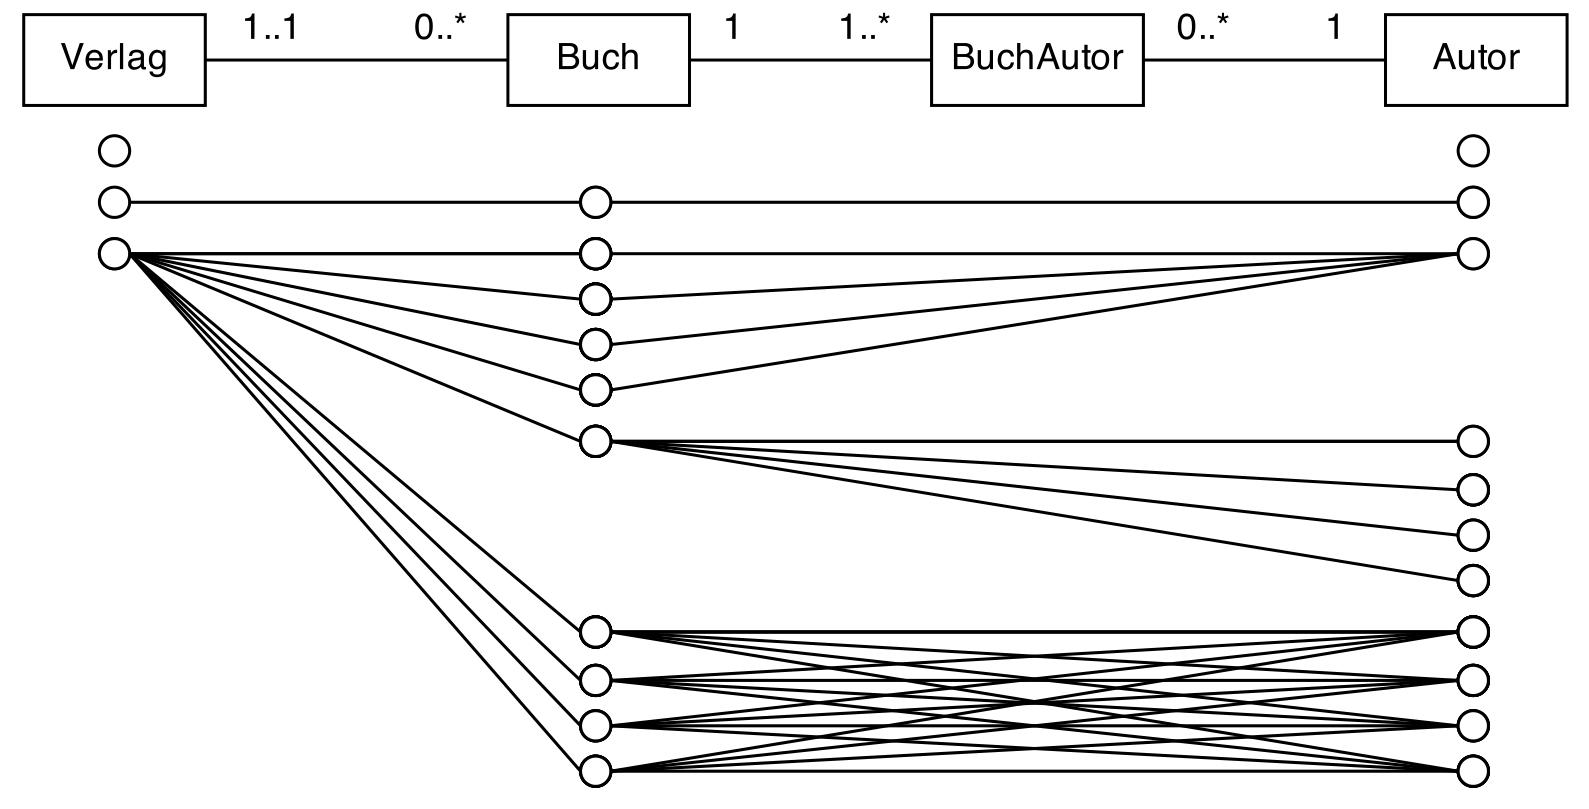
\includegraphics[width=12.75cm]{images/generiert.png}
			\caption{\label{generiert}Beispiel-Datenbankschema und daraus generierte Entitäten und Beziehungen.}
		\end{center}
	\end{figure}


Zielsetzung war die Generierung von möglichst kleinen Testdaten-Sets, die für möglichst viele fachliche Tests verwendet werden können, d.h.~eine hohe Testabdeckung bieten. 
%
%Kleine, wiederverwendbare Datasets lassen sich einfacher verstehen und erleichtern den Umgang mit Tests, da man sich  nicht immer wieder in neue Datasets hineinversetzen müssen.
%
Eine umfassende Literaturanalyse und die Evaluation existierender Werkzeuge ergab, dass bisher keine passende Lösung für diese Anforderung existiert.
%
%In der Wissenschaft beschriebene Ansätze und Algorithmen generieren meist für eine zu testende SQL-Abfrage einen passenden Testdatenbestand. Einer SQL-Abfrage liegt dabei eine formale Spezifikation zu Grunde, die allerdings für ein Anwendungsprogramm normalerweise nicht vorhanden ist. Existierende Software-Werkzeuge fokussieren sich auf die Generierung von Massendaten, die v.a. für Performanz-Tests und nicht für funktionale Tests geeignet sind. Dies zeigt sich auch daran, dass diese Werkzeuge Beziehungen zwischen Entitäten nur zufällig erzeugen und im Allgemeinen wesentlich mehr Daten generieren als für einen Menschen noch einfach verständlich sind. Weiterhin deuten Untersuchungen im Projekt darauf hin, dass die Komplexität der Testdatengenerierung im allgemeinen Fall nicht-polynomial ist.
%
Aus diesem Grund wurde ein neuer Algorithmus zur Testdatengenerierung entworfen. 
%
Anleihen konnten dabei aus \cite{Houkjaer:2006:SRD:1182635.1164254} gezogen werden.
%
Idee ist, durch Nutzung von Äquivalenz\-klas\-sen und das gezielte Generieren von Grenzfällen bei Beziehungen eine hohe Testabdeckung zu erreichen.


	




Der Algorithmus betrachtet das Datenbankschema als Graph. 
%
Tabellen stellen Knoten, Beziehungen (Fremdschlüssel) stellen Kanten dar.
%
Da assoziative Tabellen ebenfalls Beziehungen ausdrücken, werden diese als besondere Kanten behandelt. 
%
%Der Graph wird ausgehend von einem Knotens traversiert. 
%
Ausgehend von einem beliebigen Startknoten werden die Kanten und die damit verbundenen Knoten rekursiv traversiert.
%
Der Algorithmus erzeugt zu jeder Kante Entitäten der beteiligten Tabellen und mindestens Beziehungen für alle Kombinationen der unteren und oberen Grenzwerte, entsprechend den spezifizierten Unter- und Obergrenzen.
%
Gleichzeitig wird versucht, die Anzahl der generierten Entitäten und Beziehungen zu minimieren.
%
Aus diesem Grund werden auch nicht alle, über mehrere Kanten hinweg, mögliche Kombinationen berücksichtigt, da dies zu einer kombinatorischen Explosion führen würde.
% hier evtl die Grenzfälle erläutern...
%S
%Jede Kante und jede Tabelle werden genau genau einmal durchlaufen.
%Der  Algorithmus berücksichtigt lokal alle Kombinationen der unteren und oberen Grenzwerte von Beziehungstypen und versucht gleichzeitig die Anzahl der generierten Entitäten und Beziehungen zu minimieren. Globale Abhängigkeiten über mehrere Beziehungstypen hinweg, die zu einer kombinatorischen Explosion führen können, bleiben dabei (augenblicklich) unberücksichtigt. 


	
Der Algorithmus soll an dem  Datenbankschema  aus Abb.~\ref{generiert} (UML-Darstellung mit Multiplizitäten) veranschaulicht werden. 
%
%Ein Buch gehört genau zu einem Verlag und wird von beliebig vielen (mindestens einer) Autoren geschrieben. 
%Ein Verlag kann selbst beliebig viele und sogar keine Bücher veröffentlichen und ein Autor kann an keinem oder beliebig Büchern beteiligt sein.
%	
%	\begin{figure}[htb]
%		\begin{center}
%			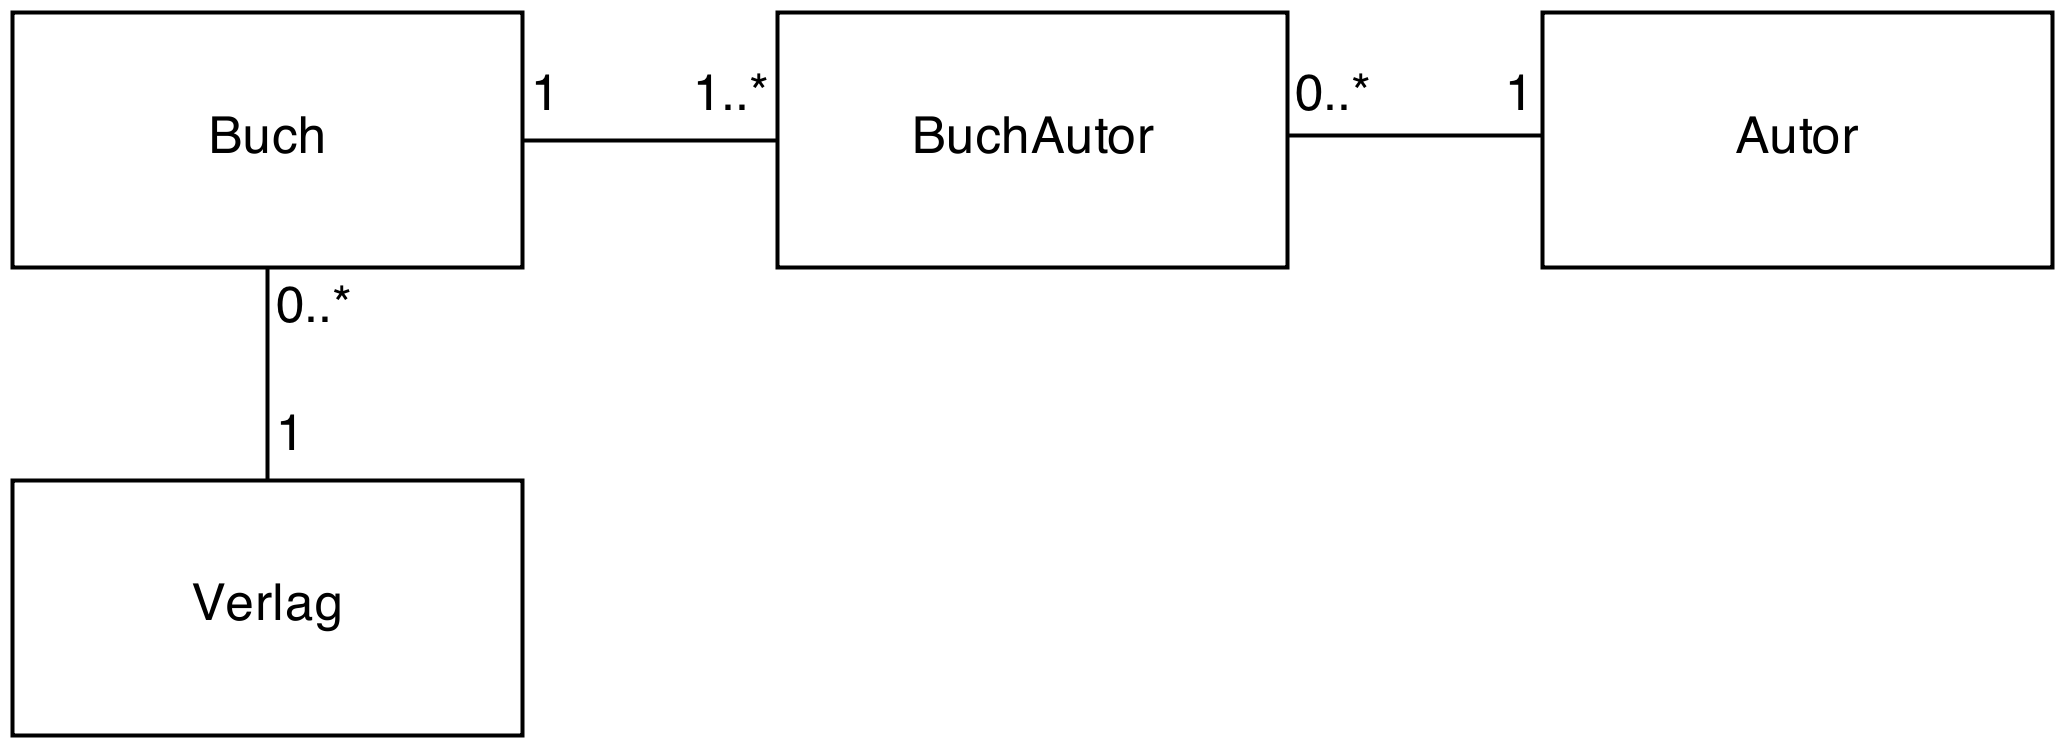
\includegraphics[width=10cm]{images/database.png}
%			\caption{\label{database}Datenbank-Schema der Bücherverwaltung}
%		\end{center}
%	\end{figure}
%	
Als Startknoten wird im Beispiel \textit{Buch} verwendet. 
%
Von hier aus werden alle Kanten besucht, hier angefangen mit der Kante (1..1:0..*) zum Knoten \textit{Verlag}. 
%
%Dieser repräsentiert eine 1:0..*-Beziehung. 
%
Um möglichst alle Grenzfälle bzw.~Äquivalenzklassen abzudecken, wird erzeugt: (1) eine Verlags-Entität, die keine Bücher verlegt, (2) ein Verlag, der genau ein Buch verlegt und (3) ein  Verlag, der viele
Bücher veröffentlicht\footnote{Für * wird ein konfigurierbarer Wert  verwendet, im Beispiel $4$.}.
%
%Für * wird ein konfigurierbarer Wert (hier: $4$) verwendet. 
%
%Für diese Kante werden also drei Entitäten des Typs Verlag und fünf Entitäten des Typs Buch erzeugt.
%	
Der Knoten \textit{Verlag} hat keine nicht-besuchten Kanten, weshalb die Traversierung in \textit{Buch} fortgesetzt wird mit der Kante zum Knoten \textit{BuchAutor} (assoziative Tabelle, die eine 0..*:1..*-Assoziation zwischen \textit{Buch} und \textit{Autor} ausdrückt). 
%
%Die Kante hat eine assoziative Tabelle als Ziel, weshalb hier andere Schritte notwendig sind wie bei der letzten Kante.
%
%Die Tabelle BuchAutor drückt eine 0..*:1..*-Beziehung zwischen Buch und Autor aus. 
%
Der Algorithmus sieht vor, die vier möglichen min/max-Kombinationen zwischen \textit{Buch} und \textit{Autor} zu generieren. 
%
Jede Beziehung zwischen einem \textit{Buch} und einem \textit{Autor} resultiert in einer Entität in der Tabelle \textit{BuchAutor}. 
%
Existierende Entitäten in \textit{Buch} und \textit{Autor} werden für diese generierten Beziehungen soweit möglich wiederverwendet, bei Bedarf werden neue Entitäten in \textit{Buch} und \textit{Autor} generiert.
%
Die Traversierung des Graph endet nun, da jede Kante besucht wurde.
%
%
%Es wird ein Autor benötigt, der kein Buch geschrieben hat, und ein Autor, der genau an einem Buch beteiligt ist (min:min). Außerdem wird ein Autor benötigt, der vier Bücher schreibt (max:min), und ein %Buch, das vier Autoren hat (min:max). Und schließlich werden vier Bücher benötigt, die jeweils die gleichen vier Autoren haben (max:max). Für die assoziative Tabelle BuchAutor werden folglich zehn Entitäten des Typs Buch und elf Entitäten des Typs Autor benötigt, wobei die bereits erzeugten Entitäten des Typs Buch hier weiterverwendet werden. 
%
%Die Traversierung endet hier, da jede Kante besucht wurde.
%
Allerdings sind einige der bis hierhin erzeugten \textit{Buch}-Entitäten noch ungültig, da sie noch nicht zu einem \textit{Verlag} gehören.
%
Solche Entitäten werden im letzten Schritt des Algorithmus behandelt. Alle Entitäten werden auf Gültigkeit bzgl.~ihrer Beziehungen überprüft und bei Bedarf werden weitere Beziehungen und weitere Entitäten erzeugt.
%
Abb.~\ref{generiert} stellt das im Beispiel generierte Testdaten-Set (Entitäten und ihre Beziehungen) grafisch dar. 
%
%Eine Entität wird als Kreis dargestellt, die Verbindungslinien zwischen den Entitäten stellen ihre Beziehungen dar. 
%
%Dazu gehören auch die genierten Entitäten in der assoziativen Tabelle BuchAutor.
	
%	Die fünf im vorausgegangenen Schritt erzeugten Entitäten des Typs Buch sind allerdings noch ungültig, da sie noch nicht zu einem Verlag
%	gehören. Solche Entitäten werden im letzten Schritt behandelt. Alle Entitäten werden auf Gültigkeit bzgl. ihrer Beziehungen überprüft,
%	und bei Bedarf werden weitere Beziehungen und falls notwendig weitere Entitäten erzeugt. Abb.~\ref{generiert} stellt die generierten
%	Entitäten und ihre Beziehungen grafisch dar. Eine Entität wird als Kreis dargestellt, die Verbindungslinien zwischen den Entitäten
%	stellen ihre Beziehungen dar. Dazu gehören auch die genierten Entitäten in der assoziativen Tabelle BuchAutor.
		
Details zum Algorithmus (Pseudocode) und zur Java-Implementierung sind in \cite{MT:Moll:2013} zu finden.
%
Evaluationen haben gezeigt, dass die generierten Testdaten unabhängig von der Reihenfolge der Traversierung und  bzgl.~des Datenbankschemas immer gültig sind.
%
Zur Erzeugung der Werte von Entitäten wurden verschiedene Wertegeneratoren implementiert.	

%	Der Algorithmus wurde in Java als Teil von STU implementiert. Details zum Algorithmus und sein Pseudo-Code, zur Implementierung und zur
%	Generierung von Daten für die einzelnen Entitäten sind in \cite{MT:Moll:2013} zu finden. Verschiedene Evaluationen haben gezeigt, dass
%	sich die erzeugten Testdaten in Unit-Tests nutzen lassen und auch in die Datenbank einspielen lassen. Das Ergebnis der Generierung ist
%	bei der aktuellen Implementierung unabhängig von der Reihenfolge der Traversierung.
	
	



\section{Fazit}

Die in dieser Arbeit vorgestellten Konzepte und die daraus resultierende Software wurden in das vorhandene STU-Framework integriert.
%
Der  Code steht  unter der Apache License 2.0 unter \texttt{https://github.com/seitenbau/stu/}  zur Verfügung. 
%

Die entwickelte Testdaten-DSL wurde bereits in der Qualitätssicherung von mehreren produktiven Softwareprojekten  eingesetzt.
%
Der Spezifikationsaufwand und die Fehlerrate konnte  im Vergleich zur  früheren Vorgehensweise  deutlich reduziert werden.
%
Der Testdatengenerator wurde dabei  auf  Datenbankschemata mit teilweise mehr als 80 Tabellen angewandt.
%
Der  Testdatengenerator konnte in jedem Fall  einen konsistenten, übersichtlichen Testdaten-Set erzeugen, der eine sehr gute Startbasis für die Anwendungstests ergab.
%Die erzeugten Testdaten-Sets boten eine sehr gute Startbasis für die Anwendungstests.

%Der  Code steht  unter \texttt{https://github.com/seitenbau/stu/} unter der Apache License 2.0 zur Verfügung. 
%
%Details zur Implementierung und ausführliche Code-Beispiele zur Verwendung sind in \cite{MT:Moll:2013} zu finden.



\bibliography{GI-IT-TD}

\end{document}



